\section{Transfert thermique et Flux}
\subsection{Les 3 Modes de transferts thermiques}

Il y a 3 manières pour un système pour recevoir du transfert thermique\footnote{on pourrait dire pour recevoir de la chaleur mais ce mot est banni pour cause de confusion avec la température}


\begin{itemize}
\item le transfert thermique \textbf{par rayonnement} : \trou{ transfert d'énergie sous forme d'ondes électromagnétiques, principalement dans l'infrarouge, émis par des objets en raison de leur température.}
\item le transfert thermique \textbf{par \trou{convection}} : l'énergie thermique se transmet de proche en proche dans un fluide avec \textbf{mouvement d'ensemble} de celui-ci.
\item le transfert thermique \textbf{par \trou{conduction}} : Il y a contact entre le système et l'extérieur. L'agitation thermique se transmet de proche en proche dans la matière \trou{sans déplacement} d'ensemble de celle-ci.\\
\begin{center}
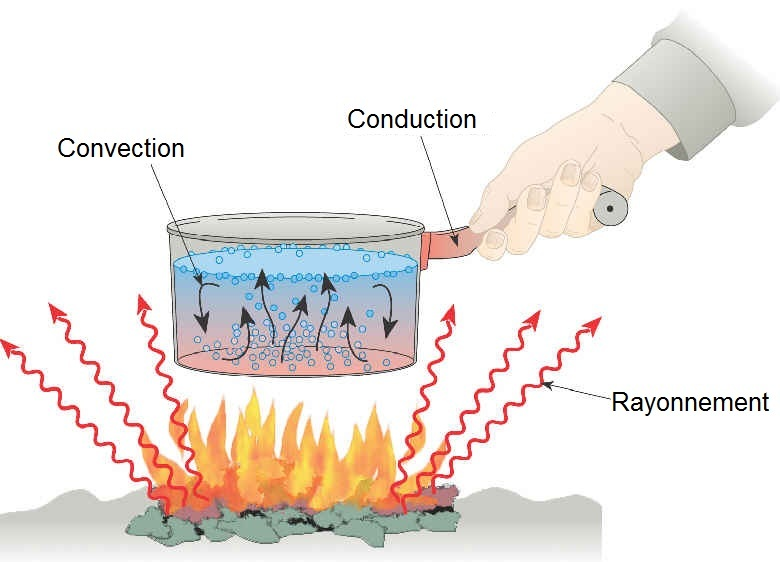
\includegraphics[scale=0.5]{figures/thermo/convection}
\end{center}
\end{itemize}

%\newpage
%\blocgris{Application}{Repérer dans le texte suivant les différents transferts thermiques et essayez de regrouper ces exemples en trois catégories : \\
%\textit{C'est le printemps, vous vous prélassez au soleil. Il fait chaud.\\
%Vous rentrez ensuite préparer votre repas. Au menu, spaghettis bolognaise. Vous placez votre casserole d'eau sur la plaque électrique. L'eau se réchauffe et commence à bouillir. Vous y plongez vos pâtes. Vous mettez la sauce bolognaise à réchauffer dans une autre casserole et vous oubliez votre cuillère en inox dedans. Au moment de remuer, impossible de toucher la cuillère, elle est bien trop chaude. Vous allez donc chercher une cuillère en bois.\\
%Une fois repus, vous vous préparez une boisson chaude. Vous mettez votre tasse au micro-onde. En trente secondes, c'est chaud. Vous entourez votre tasse de vos mains pour les réchauffer puis vous vous asseyez, le dos contre le radiateur chaud. \\
%Au moment où vous montez vous coucher, vous vous rendez compte qu'il fait bien plus chaud à l'étage qu'au rez de chaussée alors que les radiateurs ne sont allumés qu'en bas.\\
%Vous vous endormez jusqu'au petit matin où vous débuterez une nouvelle journée rythmée par les transferts thermiques.}
%}
%\newpage
\subsection{Le flux thermique}
\etiquette{Contexte} On considère une paroi qui sépare deux milieux de températures différentes $T_1$ et $T_2$ telle que $T_1>T_2$. L'écart de température provoque de la \trou{conduction} entre la face chaude et la face froide. On dit qu'un flux\footnote{flux vient du latin fluxus qui signifie écoulement} thermique noté $\Phi$ traverse la paroi. Ce flux est une \trou{puissance} elle s'exprime donc en Watt de symbole \trou{W}.


\begin{center}
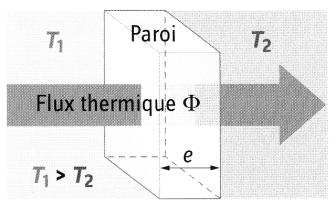
\includegraphics[scale=0.5]{figures/thermo/fig1}
\end{center}


\etiquette{Interprétation Physique} $\Phi$ représente l'énergie qui traverse la paroi chaque seconde. $$\boxed{1\:W = 1 \:J/s}$$

\subsection{Résistance thermique}
\begin{itemize}
	\item Plus l'écart de température est grand et plus la conduction est \trou{importante}, plus $\Phi$ est \trou{grand}.
	\item Le flux dépend du matériau qui constitue la paroi et des dimensions de la paroi. On parle alors de la \trou{résistance thermique de la paroi}, elle se note $R_{th}$.
\end{itemize}

\blocrouge{Formules}{$$\Phi=\frac{T_1 - T_2}{\trou{R_{th}}}$$ Unités: $\Phi$ en W (ou J/s) ; $T_1$, $T_2$ en K ; $R_{th}$ en K/W $$R_{th}=\frac{\trou{ e }}{\lambda . S}$$ Unités: e: en m ; $S$ en $m^2$ et $\lambda$: conductivité thermique de la paroi en $\SI{}{\watt\per\kelvin\per\meter}$
}

\etiquette{Conséquences}
\begin{itemize}
	\item Le flux est d'autant plus grand que la résistance thermique $\rm R_{th}$ est \trou{petite}.
	\item Ce flux est d'autant plus grand que la différence de température $\rm T_1-T_2$ est \trou{grande}
	\item Plus l'épaisseur de la paroi est grande, plus sa résistance thermique est \trou{grande} et plus elle est isolante/conductrice.
	\item Plus la surface de la paroi est grande, plus sa résistance thermique est \trou{petite.}
\end{itemize}



\blocgris{Exercice}{On considère un mur en béton de surface 10 $m^2$ et d'épaisseur 15 cm. Ce mur sépare l'intérieur d'une habitation dont la température est \SI{20}{\celsius} et l'extérieur dont la température est $5^\circ$C. La conductivité thermique du béton est $\SI{0,013}{\watt\per\kelvin\per\meter}$.
\begin{enumerate}
	\item Calculer la résistance thermique du mur.
	\item En déduire le flux thermique traversant le mur.
\end{enumerate}
%\vspace{7  cm}
}

\begin{travail}
\begin{itemize}
	\item Résistance thermique: \url{https://labolycee.org/isolation-thermique-du-rover-perseverance}
	\item Application du premier principe: \url{https://labolycee.org/linteret-energetique-dune-pac}
	\item Autre sujet de bac: \url{https://labolycee.org/le-sauna}
\end{itemize}

\end{travail}


\section{Température terrestre moyenne}

\subsection{Corps Noir et Rayonnement Thermique}

Le rayonnement thermique du Soleil et de la Terre sont très bien décrits par le modèle du \textbf{corps noir}. Ce modèle décrit la production de rayonnement thermique sous l'effet de la température.

\etiquette{Loi de Stefan-Boltzmann} La puissance rayonnée par unité de surface par un corps noir vaut :
$$\boxed{P=\sigma\ T^4}$$

où $\sigma = \SI{5,67e-8}{W.m^{-2}.K^{-4}}$ est la \textbf{constante de Stefan-Boltzmann}.

\subsection{Hypothèses du modèle simplifié}

\begin{itemize}
	\item La Terre est à \textbf{l'équilibre thermique} : l'énergie reçue = l'énergie émise
	\item La Terre se comporte comme un \textbf{corps noir de température $T$}
	\item Le système Terre-Atmosphère reçoit une puissance solaire moyenne par unité de surface : $$P_S= \SI{340}{W.m^{-2}}$$
	\item Une fraction $A$ de cette puissance est \textbf{réfléchie} (albédo terrestre) : $$A=0,34$$
	\item La puissance surfacique \textbf{absorbée} par la Terre vaut donc : $$P_{absorbee}= (1-A)\times P_S$$
	\item \textbf{L'atmosphère} absorbe une fraction $a=0,45$ du rayonnement infrarouge émis par la surface terrestre et le \textbf{renvoie partiellement vers la surface} (effet de serre)
\end{itemize}

\subsection{Schéma du bilan énergétique}
\begin{center}
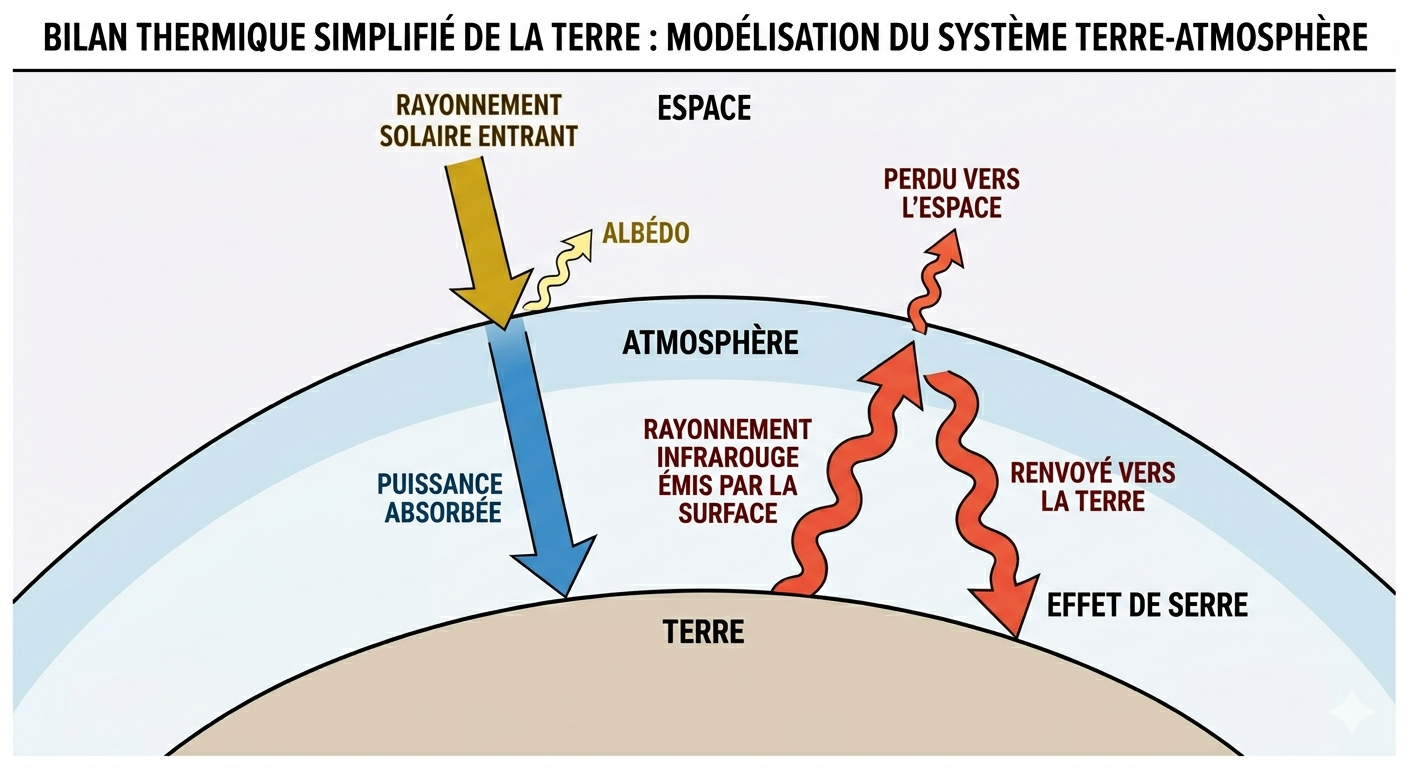
\includegraphics[width=.7\textwidth]{figures/thermo/albedo.png}
\end{center}
\subsection{Bilan énergétique sans atmosphère}

En l'absence d'atmosphère, la Terre ne reçoit que le rayonnement solaire et émet uniquement vers l'espace.

\etiquette{Équilibre thermique} À l'équilibre :
$$P_{absorbee} = P_{emise}$$

$$(1-A) \times P_S = \sigma T_0^4$$

\etiquette{Calcul} En isolant la température :
$$T_0 = \left[\frac{(1-A) \times P_S}{\sigma}\right]^{1/4}$$

$$T_0 = \left[\frac{0,66 \times 340}{5,67 \times 10^{-8}}\right]^{1/4} = \left[\frac{224}{5,67 \times 10^{-8}}\right]^{1/4}$$

$$\boxed{T_0 \approx \SI{255}{K} = \SI{-18}{\celsius}}$$

\etiquette{Interprétation} Sans atmosphère, la Terre serait gelée à $-18°C$ !

\subsection{Bilan énergétique avec atmosphère : l'effet de serre}

L'atmosphère absorbe une fraction $a = 0,45$ du rayonnement infrarouge émis par la Terre et le \textbf{renvoie partiellement vers la surface}. Cela génère un surplus d'énergie à la surface.

\etiquette{Nouveau bilan} À l'équilibre (incluant le retour de l'IR par l'atmosphère) :
$$(1-A) \times P_S + \text{(rayonnement renvoyé par l'atmosphère)} = \sigma T^4$$

Le rayonnement renvoyé par l'atmosphère crée un \textbf{effet de serre} qui augmente la température.

\etiquette{Résultat qualitatif} L'inclusion de cet effet de serre augmente considérablement la température terrestre :

$$\boxed{T \approx \SI{288}{K} = \SI{15}{\celsius}}$$

Cette température correspond à la \textbf{température réelle moyenne de la Terre} !

\etiquette{Différence observée}
$$\Delta T = T - T_0 = 288 - 255 = \SI{33}{K}$$

Cette différence de \textbf{33 K} est directement due à l'\textbf{effet de serre atmosphérique}.

\subsection{Influence de l'albédo et de l'effet de serre sur la température}

\etiquette{Dépendance à l'albédo} La température dépend de l'albédo selon :
$$T \propto (1-A)^{1/4}$$

\begin{itemize}
	\item Si l'albédo $A$ \textbf{augmente} (plus de nuages, plus de glace) $\Rightarrow$ moins d'énergie absorbée $\Rightarrow$ \trou{température diminue}
	\item Si l'albédo $A$ \textbf{diminue} (fonte des glaces) $\Rightarrow$ plus d'énergie absorbée $\Rightarrow$ \trou{température augmente}
\end{itemize}

\etiquette{Dépendance à l'effet de serre}

Si la concentration en \textbf{CO$_2$ augmente} $\Rightarrow$ l'atmosphère absorbe davantage l'infrarouge terrestre $\Rightarrow$ \trou{température augmente}
%
%\blocgris{Boucles de rétroaction}{
%\begin{itemize}
%	\item \textbf{Rétroaction positive} : Fonte de glace $\downarrow A$ $\Rightarrow$ absorb. $\uparrow$ $\Rightarrow$ chauffage $\uparrow$ $\Rightarrow$ fonte $\uparrow$ (amplifie)
%	\item \textbf{Rétroaction négative} : Aérosols volcaniques $\uparrow A$ $\Rightarrow$ absorb. $\downarrow$ $\Rightarrow$ refroidissement $\downarrow$ (compense)
%\end{itemize}
%}

\blocrouge{Conclusion}{

Le modèle simple du corps noir montre que la \textbf{température terrestre dépend de deux facteurs clés} :

\begin{enumerate}
	\item \textbf{L'albédo} : contrôle l'énergie solaire absorbée
	\item \textbf{L'effet de serre} : déterminé par la composition atmosphérique (CO$_2$, H$_2$O, CH$_4$)
\end{enumerate}

Les changements climatiques actuels résultent de la \textbf{combinaison} de ces deux effets : augmentation de l'effet de serre (CO$_2$ anthropique) et diminution de l'albédo (fonte des calottes glaciaires).}

\etiquette{Exercice} \url{https://www.labolycee.org/temperature-moyenne-de-surface-de-la-terre}
\section{Loi phénoménologique de Newton : transfert conducto-convectif}
\subsection{Situation}

On considère un objet de température T et de surface extérieure S. Ce système est immergé dans un fluide de température fixe $Te\neq T$.
Les températures étant différentes, on observe un transfert thermique entre le système et l'extérieur.

\begin{center}
	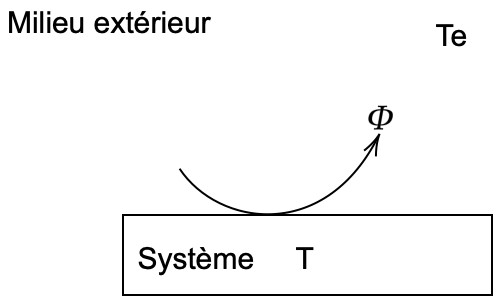
\includegraphics[scale=0.35]{figures/thermo/convection1.png}
\end{center}

\etiquette{Exemple} Plat chaud qui sort du four et qui refroidit dans l'air de la cuisine.

\etiquette{Vocabulaire}

Proche de la surface du système, le fluide touche le système. Il y a alors \textbf{conduction} mais aussi \textbf{convection} car le fluide est en mouvement. On parle de transfert \textbf{convectif} entre le fluide et la surface du système.

\blocrouge{Formule de Newton}{Le flux convectif $\Phi$ échangé entre un système à la température T et un fluide à la température Te vaut: $$\boxed{\Phi = h\times(T_e - T)\times S}$$ Unités: h est le coefficient convectif en $\SI{}{\watt\per\meter\squared\per\kelvin\squared}$ ; S: la surface du système en $m^2$ ; T et Te en K (ou\SI{}{\celsius}) et $\Phi$ en W  }


\etiquetterouge{Réfléchir au signe !}
$\Phi$ peut être positif ou négatif. Si la surface est plus chaude que l'extérieur $T_e < T$ , le flux $\Phi$ est \trou{ négatif}. Cela correspond  à une \trou{perte d'énergie} pour la surface.
On retrouve la convention de la thermodynamique et celle du banquier.
\subsection{Bilan d'énergie du système}
\etiquette{Situation}
Le système est incompressible, au repos à la température T. Il échange de l'énergie uniquement par transfert conducto-convectif avec le milieu extérieur de température Te. Condition initiale: on sait que à t=0 $T(0)=T_0$.\\

\begin{center}
	\includegraphics[scale=0.4]{figures/thermo/convection2.pdf}
\end{center}

D'après le premier principe de la thermodynamique, on a :
\trou{$\Delta U = Q$}\\
Or, $$Q=\trou{\Phi \Delta t}$$ et $$\Delta U = \trou{C.\Delta T}$$


\blocgris{A Savoir Faire}{\textbf{Etablir l'équation différentielle}. T(t) est la fonction recherchée.
\begin{align*}
	C.\Delta T &= \Phi . \Delta t & \text{Bilan\: d'énergie}\\
		C.\Delta T &=  h.(T_e-T).S .\Delta t& \text{Loi de Newton}\\
	C. \frac{\Delta T}{\Delta t} &= \Phi = h.(T_e-T).S & \text{Division par }\Delta t\\
	\text{En faisant tendre \trou{$\Delta t$ vers 0}}\\
	C.\frac{dT}{dt} &= 	h.(T_e-T).S\\
	\\
	\frac{dT}{dt} &= 	\frac{h.S}{C}(T_e-T)\\
	\\
	\boxed{\dfrac{dT}{dt}=-\dfrac{hS}{C}T + \dfrac{hS}{C}Te} & &\text{Mise sous la forme }y'=ay+b
\end{align*}
}

On obtient une équation différentielle d'ordre 1 avec second membre constant.\\

\etiquette{Solution de l'équation différentielle}

\begin{center}
\trou{$$\boxed{T(t)=Te+(T_0-Te)e^{-t/\tau}}$$}
\trou{Avec $\tau=\dfrac{C}{hS}$ le temps caractéristique de refroidissement, exprimé en seconde}
\end{center}

Vérifier que cette expression est bien solution de l'équation différentielle et que $\tau$ est bien homogène à un temps.

\begin{travail}
\begin{itemize}
	\item Asie 2024 Jour 1  \url{https://www.labolycee.org/etude-dune-bouteille-isotherme}
	\item \url{https://www.labolycee.org/preparer-un}
\item \url{https://www.labolycee.org/capacite-thermique-massique-du-cuivre}
\item \url{https://www.labolycee.org/evolution-de-la-temperature-dans-une-bouteille-isotherme}

\end{itemize}
\end{travail}
